%Пупупум
%вечер добрый
\begin{theorem} \hypertarget{thrm2.1}{(Дифференцируемость сложной функции)}
    Пусть $G \subset \R^n$~---~открыто и непусто, $\Omega \subset \R^m$~---~открыто и непусто. $F: G \rightarrow \Omega$ дифференцируемо в точке $x^0 \in G, H: \Omega \rightarrow \R^d$ дифференцируемо в точке $y^0 = F(x^0) \in \Omega$. Тогда для композиции $\phi = H \circ F$, якобиан будет равен: $J_\phi(x^0) = \D(H \circ F)(x^0) = \D H(F(x^0)) \D F(x^0)$, а $\frac{\partial \phi_i}{\partial x_j} = \sum \limits_{k = 1}^m \frac{\partial H_i}{\partial y_k} \cdot \frac{\partial F_k}{\partial x_j}, i \in \{1, \dots, d\}, j \in \{1, \dots, n\}$
\end{theorem}

\begin{proof}
    Так как $F$ дифференцируема в точке $x^0 \in G$, можем записать, а $H$ дифференцируема в точке $y^0 \in H$: $$ F(x) - F(x^0) = \D F(x^0) \cdot (x - x^0) + o(||x - x^0||)\quad(*)$$
    $$H(y) - H(y^0) = \D H(y^0)\cdot (y - y^0) + o(||y - y^0||)$$
    Так как $F$ -- дифференцируема в точке $x^0 \Rightarrow$ непрерывна в точке $x^0$. Тогда, если $x$ в достаточно малой окрестности точки $x^0$, то $F(x)$ попадает в достаточно малую окрестность $y^0 = F(x^0)$. Подставим $F(x^0)$ вместо $y^0$. $$H(F(x)) - H(F(x^0)) = \D H(F(x^0))\left[\D F(x^0)(x - x^0) + o(||x - x^0||)\right] + \epsilon_{y^0}(y)|| F(x) - F(x^0)|| = $$ $$ = \D H(F(x^0))\left[\D F(x^0)(x - x^0) + o(||x - x^0||)\right] + \epsilon_{y^0}(y)\cdot||(*)|| = $$ $$ = \D H(F(x^0)) \D F(x^0)(x - x^0) +\D H(F(x^0))o(||x - x^0||) + \epsilon_{y^0}(F(x)) \big|\big| \D F(x^0)(x - x^0) + o(||x - x^0||)\big|\big|$$
    Заметим, что: $\D H(F(x^0)) \cdot o(||x - x^0||) = o(||x - x^0||)$, так как точка зафиксирована, матрица($d \times m$) домножается на столбец (высоты $m$) и получается столбец (высоты $d$). \newline 
    Обозначим как $I = \epsilon_{y^0}(F(x))\big|\big|\D F(x^0)(x - x^0) + o(||x - x^0||)\big|\big|$. Докажем, что $I = o(||x - x^0||)$: $$|I| \leq \big|\epsilon_{y^0}(F(x))\big| \ ||\D F(x^0)(x - x^0)|| + \big |\epsilon_y F(x) \big| \ \big|\big|o(||x - x^0||)\big|\big| $$
    Данное неравенство верно по неравенству треугольника для норм. 
    Вторая часть суммы очевидно равна $o(||x - x^0||)$. Докажем, что первая часть суммы также равна $o(||x - x^0||)$. Обозначим за $y$ итоговый столбец произведения. Тогда: $$|y_i| = \sum\limits_{i = 1}^n |\D F(x^0)_{i, j}| \ |(x_j - x^0_j)| \leq \sum\limits_{i = 1}^n |\D F(x^0)_{i, j}| \ ||x - x^0|| \Rightarrow $$ $$ ||y|| = \sum\limits_{i = 1}^m |y_i|^2 \leq \sqrt{m} (\sum\limits_{i = 1}^m |y_i| = \sqrt{m}(\sum\limits_{i = 1}^n \sum\limits_{j = 1}^m \D F(x^0)_{i, j} \cdot ||x - x^0|| = o(||x - x^0||)$$
    В итоге получаем, что $H(F(x)) - H(F(x^0)) = \D H(F(x^0)) \cdot \D F(x^0)(x - x) + o(||x - x^0||)$
\end{proof}
\begin{corollary} 
    Инвариантность формы первого дифференциала
    Пусть $G \subset \R^n, \Omega \subset \R^m$~---~открытые и непустые. $F : G \rightarrow \Omega$~---~дифференцируема в $x^0$, $H: \Omega \rightarrow \R^d$~---~дифференцируема в точке $y^0 = F(x^0)$. Обозначим $y = F(x), z = H(y)$. Тогда $d(H \circ F) = dz = \D H(y^0)dy$ имеет ту же форму записи, что и дифференциал отображения $z = H(y)$. Только в первом случае, $dy$~---~дифференциал отображения $y = F(x)$ в точке $x^0$, а во втором~---~вектор приращений $y$.
    \begin{proof}
        $$d_{x^0}(H\circ F) = \D(H \circ F)(x^0)(x - x^0) \Rightarrow dy = d_{x^0}F = \D F(x^0) dx$$
        По предыдущей теореме $H \circ F$~---~дифференцируемо в точке $x^0$ и $\D (H\circ F)(x^0) = \D H(F(x^0)) \cdot \\ \cdot \D F(x^0) \Rightarrow d_{x^0}(H \circ F) = dz = \D H(F(x^0)) \D F(x^0)dx$. С другой стороны, если рассматривать $z = H(y)$, то $dz = \D H(F(x^0)) dy$. 
        Аналогично одномерному случаю, дифференциал второго порядка, не будет иметь инвариантности формы записи. 
    \end{proof}
\end{corollary}
\subsection{Частные производные высших порядков}
\begin{definition}
    Пусть $G \subset \R^n$~---~открыто и непусто, $F$: $G \rightarrow R$. Пусть $\frac{\partial f}{\partial x_i}(x)$~---~существуют для $\forall x \in G$. Тогда если в точке $x^0 \in G$ существует частная производная по $j$-ой координате от функции $\frac{\partial f}{\partial x_i}$, то она обозначается $\frac{\partial^2f}{\partial x_j \partial x_i}(x^0)$. Пусть теперь при некотором $m \in \N$ определена в $G$ функция $\frac{\partial^{m -1}f}{\partial x_{i_2} \dots \partial x_{i_m}}, \ i_2, \dots, i_m \in \{1, \dots n\}$, тогда если $i_1 \in \{1, \dots, n\}$, то $\frac{\partial^mf}{\partial x_{i_1}\dots\partial x_{i_m}}(x^0) := \frac{\partial}{\partial x_{i_1}}\left(\frac{\partial^{m - 1}f}{\partial x_{i_2}\dots \partial x_{i_m}}\right)$.
\end{definition}
\begin{note}
    В общем случае частные производные не коммутируют.
\end{note}
\begin{example}
    \begin{equation*}
        f(x, y) = 
        \begin{cases}
            xy\frac{y^2 - x^2}{x^2 + y^2} & x^2+y^2 \neq 0 \\
            0 & x^2 + y^2 = 0
        \end{cases}
    \end{equation*}
    Покажем, что: 
    $
        \begin{cases}
             \exists \frac{\partial^2f}{\partial x \partial y}(0, 0) \\ 
             \exists \frac{\partial^2f}{\partial y \partial x}(0, 0)
        \end{cases}
    $ и они неравны
    $$\frac{\partial f}{\partial x} =\frac{\partial}{\partial x}\left(xy \frac{y^2 - x^2}{x^2 + y^2}\right) = y \frac{y^2 - x^2}{x^2 + y^2} + xy
    \left[\frac{2x}{x^2 + y^2} - \frac{y^2 - x^2}{(x^2 + y^2)^2}\cdot 2x\right]$$
    $$\dfrac{\partial f}{\partial y} = \frac{\partial}{\partial y}\left(xy \frac{y^2 - x^2}{x^2 + y^2}\right) = x \frac{y^2 - x^2}{y^2 + x^2} + xy\left[ \frac{2y}{x^2 + y^2} - 2y \frac{y^2 - x^2}{(x^2 + y^2)^2}\right]$$
    Данные выражения справедливы для $x^2 + y^2 \neq 0$. Посчитаем по определению частные производные для точек, где $x^2 + y^2 = 0$: посмотрим на вид функции (срез) при $x = 0$ или при $y = 0$. Она будет равна нулю в этих точках. Тогда: $\frac{\partial f}{\partial x} = \frac{\partial f}{\partial y} = 0$ при $x^2 + y^2 = 0$.
    $$\frac{\partial^2 f}{\partial y \partial x}(0, 0):= \lim \limits_{y \rightarrow 0} \dfrac{\frac{\partial f}{\partial x} (0, y)- \frac{\partial f}{\partial x}(0, 0)}{y} = \lim \limits_{y \rightarrow 0} \dfrac{\frac{\partial f}{\partial x}(0, y)}{y} = \lim \limits_{y \rightarrow 0} \dfrac{y^2}{y^2} = 1$$
    $$\frac{\partial^2 f}{\partial x \partial y}(0, 0) := \lim \limits_{x \rightarrow 0}\dfrac{\frac{\partial f}{\partial y}(x, 0) - \frac{\partial f}{\partial y}(0, 0)}{x} = \lim \limits_{x \rightarrow 0}\dfrac{\frac{\partial f}{\partial y}(x, 0)}{x} = \lim \limits_{x \rightarrow 0}\dfrac{-x^2}{x^2} = -1$$
    Видим, что частные производные существуют, но не равны.
\end{example}
\begin{theorem} \hypertarget{thrm2.2}{}
    Пусть $G \subset \R^2$~---~открыто и непусто. Пусть для $\forall x, y \in G \begin{cases}
        \exists \frac{\partial^2 f}{\partial x \partial y}(x, y) \in \R \\ 
        \exists \frac{\partial^2 f}{\partial y \partial x}(x, y) \in \R
    \end{cases}$. Тогда если $\frac{\partial^2 f}{\partial x \partial y}$ и $\frac{\partial^2 f}{\partial y \partial x}$ непрерывны в точке $(x^0, y^0) \in G$, то они равны в этой точке. 
\end{theorem}
\begin{proof}
    Фиксируем точку $(x^0, y^0) \in G$, в которой функция непрерывна. Поскольку множество открытое, то $\exists \delta > 0$: $B_\delta(x^0) \subset G \Rightarrow \exists \widetilde{\delta} > 0$: $[x^0 - \widetilde{\delta}$, $x^0 + \widetilde{\delta }] \times [y^0 - \widetilde{\delta}$, $y^0 + \widetilde{\delta}] \subset B_{\delta}(x^0) \subset G$. Можно взять $\widetilde{\delta} = \frac{\delta}{1 + \sqrt{2}}$.
    \begin{center}
        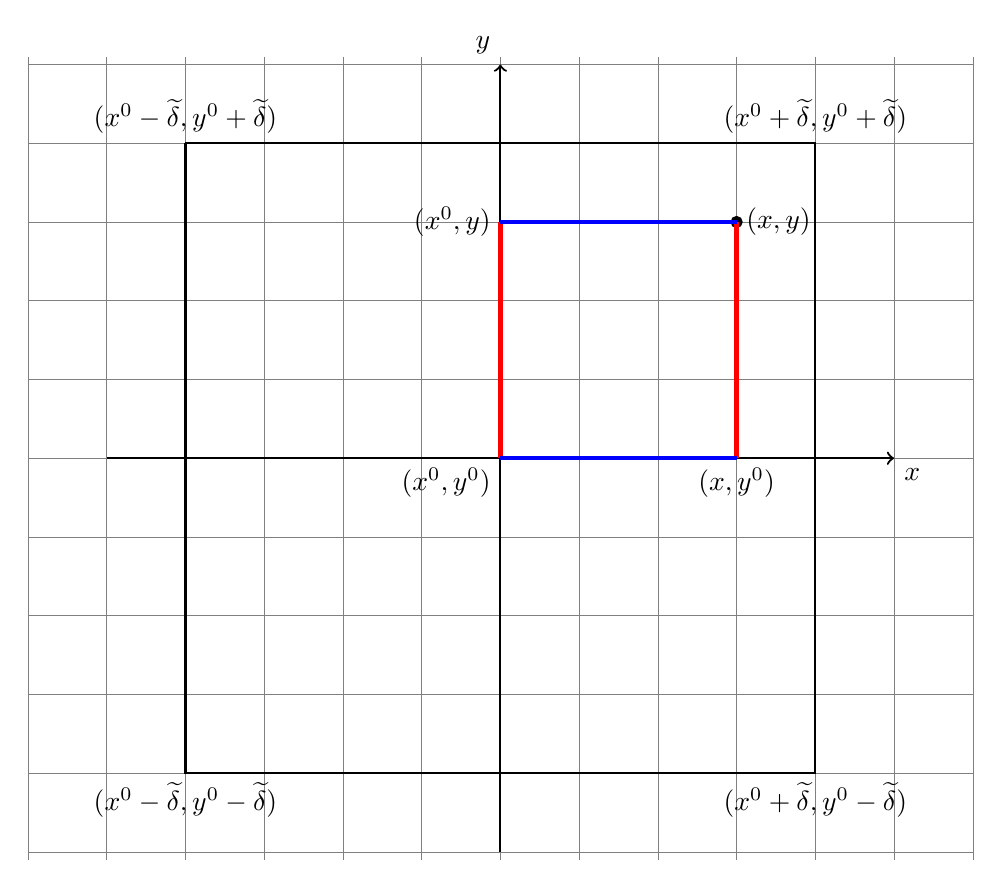
\begin{tikzpicture}
            \draw[step=1cm,gray,very thin] (-6,-5.1) grid (6,5.1);
            \draw[thick,->] (-5 ,0) -- (5,0) node[anchor=north west] {$x$};
            \draw[thick,->] (0,-5) -- (0, 5) node[anchor=south east] {$y$};
            \draw[thick] (-4, 4) -- (4, 4) -- (4, -4) -- (-4, -4) -- (-4, 4);
            \draw (-4, 4) node [anchor=south]{$(x^0 - \widetilde{\delta}, y^0 +  \widetilde{\delta})$};
            \draw (4, 4) node [anchor=south]{$(x^0 + \widetilde{\delta}, y^0 +  \widetilde{\delta})$};
            \draw (4, -4) node [anchor=north]{$(x^0 + \widetilde{\delta}, y^0 -  \widetilde{\delta})$};
            \draw (-4, -4) node [anchor=north]{$(x^0 - \widetilde{\delta}, y^0 -  \widetilde{\delta})$};
            \filldraw[black] (3,3) circle (2pt) node[anchor=west]{$(x, y)$};
            \draw (0, 0) node [anchor=north east]{$(x^0, y^0)$};
            \draw[ultra thick, red] (3, 3) -- (3, 0) ;
            \draw[ultra thick, red] (0, 3) -- (0, 0) ;
            \draw[ultra thick, blue] (3, 3) -- (0, 3);
            \draw[ultra thick, blue] (3, 0) -- (0, 0);
            \draw (3, 0) node [anchor=north ]{$(x, y^0)$};
            \draw (0, 3) node [anchor= east]{$(x^0, y)$};
        \end{tikzpicture}
    \end{center}

    \noindent Рассмотрим произвольную точку $(x, y)$ из этого квадрата (разность красных планок)
    $$\left[f(x, y) - f(x, y^0)\right] - \left[f(x^0, y) - f(x^0, y^0)\right]$$ Обозначим $\phi(x) = f(x, y) - f(x, y^0)$. Тогда записанное выше выражение будет выглядеть как $\phi(x) - \phi(x^0)$. Заметим, что при фиксированных $y$, $y^0$, $\forall x \in (x^0 - \widetilde{\delta}$, $x^0 + \widetilde{\delta}), \phi$ дифференцируема в точке $x$. Также $\phi$ непрерывна на отрезке $[x^0 - \widetilde{\delta}, x^0 + \widetilde{\delta}]$. 
    \noindent По теореме Лагранжа о среднем $\exists \theta_1(x, y) \in (0, 1)$: $\phi(x) - \phi(x^0) = \phi'(x^0 + \theta_1(x, y) \cdot (x - x^0))(x - x^0)$. В то же время $ \phi'(x^0 + \theta_1 \cdot (x - x^0)) = \left[\frac{\partial f}{\partial x}(x^0 + \theta_1(x - x^0), \ y) - \frac{\partial f}{\partial x}(x^0 + \theta_1(x - x^0), \ y^0)\right](x - x^0)$. Мы можем применить теорему Лагранжа о среднем второй раз для разности в квадратных скобках, в этом случае уже для $\phi'$. Тогда запишем как выглядит $\phi''$ из теоремы Лагранжа $\exists \theta_2(x, y): \phi''(x, y) 
    = \frac{\partial^2 f}{\partial y \partial x}(x^0 + \theta_1(x - x^0), \ y^0 + \theta_2(y - y^0))(x - x^0)(y - y^0)$

    \noindent В итоге $\left[f(x, y) - f(x, y^0)\right] - \left[f(x^0, y) - f(x^0, y^0)\right] = $
    \begin{flushright}
    $ = \frac{\partial^2 f}{\partial y \partial x} \left(x^0 + \theta_1(x - x^0), y^0 + \theta_2(y - y^0)\right)(x - x^0)(y - y^0)$.
    \end{flushright}
    Рассмотрим $x = x^0 + t, y = y^0 + t, t \in (0, \widetilde{\delta})$. $$\omega(t) = \frac{\left[f(x^0 + t, y^0 + t) - f(x^0 + t, y^0)] - [f(x^0, y^0 + t) - f(x^0, y^0)\right]}{t^2} = \frac{\partial^2 f}{\partial y \partial x}(x^0 + \theta_1t, y^0 + \theta_2t)$$
    Заметим, что если мы поменяем местами $x$ и $y$, то получим симметричную ситуацию. Вместо разности вертикальных <<планок>>, мы берем разность горизонтальных планок. Перегруппируем слагаемые (получим из тех же членов разность синих планок): 
    $$[f(x, y) - f(x^0, y)] - [f(x, y^0) - f(x^0, y^0)]$$
    Аналогично предыдущим действиям, обозначим $\psi(y) = f(x, y) - f(x^0, y)$. Тогда записанное выше выражение примет вид $\psi(y) - \psi(y^0)$. Также, дважды применим теорему Лагранжа, как для $\phi(x)$, получим, что $\omega(t) = \frac{\partial^2 f}{\partial x \partial y}(x^0 + \bar \theta_1t, y^0 + \bar\theta_2t) \longrightarrow \frac{\partial^2f}{\partial x \partial y}(x^0, y^0)$ при $t \rightarrow 0$(Именно для этого мы требуем непрерывность в точке). При этом, из действий с $\phi(t)$ мы получаем, что $\omega(t) = \frac{\partial^2f}{\partial y \partial x}(x^0 + \theta_1 t, y^0 + \theta_2 t) \longrightarrow \frac{\partial^2f}{\partial y \partial x}(x^0, y^0)$. Но при $\forall t \neq 0 \ \omega(t) = \omega(t)(\text{По постороению омеги она одинакова, при исследованни по x и по y}) \Rightarrow \frac{\partial^2 f}{\partial x \partial y}(x^0, y^0) = \frac{\partial ^ 2 f}{\partial y \partial x}(x^0, y^0)$. Тк функция $\omega(t)$ имеет предел и мы получили два значения. Такое может быть только когда ониравны
\end{proof} 
\begin{note}
    Теорема справедлива и в случае $n > 2$ переменных. То есть, если $\exists \frac{\partial^2 f}{\partial x_i \partial x_j}(x)$ и $\exists \frac{\partial^2 f}{\partial x_j \partial x_i}(x) \ \forall x \in G$ и они непрерывны в некоторой $x^0 \in G$, то они равны в этой точке. 
\end{note}
\begin{note}
    Это условие является достаточным, но не необходимым, то есть из совпадения не следует непрерывность.
\end{note}
\begin{definition}
    Пусть $G \subset \R^n$~---~непусто и открыто. Пусть фиксировано $k \in \N$. Будем говорить, что $f \ k$ \textit{раз дифференцируема в точке} $x^0 \in G $, если все частные производные порядка $k - 1$ существуют в открытом множестве $G$ и являются дифференцируемыми функциями в точке $x^0$. 
\end{definition}